\documentclass{article}
\usepackage{amsmath}
\usepackage{amssymb}
\usepackage{amsthm}
\usepackage{booktabs}
\usepackage{graphicx}

% Define your theorem-like environments
\newtheorem{theorem}{Theorem}
\newtheorem{proposition}{Proposition}

% Override the default QED symbol if you want to explicitly force the open square
\renewcommand{\qedsymbol}{\ensuremath{\square}}

\title{The Twiddle Constants, Proved and Not Copied}
\author{Douglas Quigg (dstroy0) \small dquigg123@gmail.com \\
\small This work is licensed under a \\
\small Creative Commons Attribution 4.0 International License (CC BY 4.0).
\small \date{\today}}


\begin{document}

\maketitle

\begin{abstract}
A number-theoretic transform is correct only if its modulus is prime and its twiddle root has order exactly the transform length. In the formal-verification literature those two facts are hypotheses a correctness proof rests on, established once for a standardized parameter set or supplied to the checker. This note shows them proved directly instead, by a check cheap enough to run before the transform: one Proth witness for primality, two exponentiations for the order, on unbounded integers at any width. The check is deterministic, and its verdict coincides with the probabilistic primality test the field runs at every modulus of Proth shape, with a witness in place of a confidence. A root of half the required order is shown passing every invariant computable from the twiddle table in \(O(n)\), with the order test the only one that separates it. Two silent wrong answers the check caught in one implementation are shown: a composite modulus of the correct Proth shape accepted without a primality certificate, and a 32-bit overflow on a device transform. A public artifact reproduces the certificate, both rejections and the half-order case.
\end{abstract}

\section{A number-theoretic transform trusts its constants}

A number-theoretic transform of a sequence of length \(n\) over the integers modulo \(q\) is
\[
\hat{p}_j = \sum_i p_i \, \omega^{ij},
\]
where \(\omega\) is an \(n\)-th root of unity modulo \(q\). The powers of \(\omega\) the butterflies evaluate are the \textbf{twiddle constants}. In the Cooley-Tukey butterfly they enter as \(c = a + b\omega\) and \(d = a - b\omega\); in the Gentleman-Sande butterfly as \(c = a + b\) and \(d = (a-b)\omega\). A transform of length \(2^k\) is \(k\) stages of \(n/2\) butterflies. The twiddles are touched more often than any other value in the computation, and they are the only inputs supposed to be constant.

Everything the transform computes depends on that constant having exactly the order it is supposed to have. If the modulus is not prime, or the root has an order shorter than \(n\), the transform still runs. It returns a value of the ordinary shape carrying far less structure than it should, and nothing downstream raises an error, because a wrong twiddle is not detected, it is used. Ravi, Yang, Bhasin, Zhang and Chattopadhyay make this a fault attack: a single electromagnetic fault that sets a twiddle to zero collapses the output entropy enough to recover a Kyber key and to forge a Dilithium signature, including a bypass of Dilithium's own verification.

\section{What the verification literature proves, and what it leaves open}

The correctness of a transform implementation is now machine-checked work. Hwang, Liu, Seiler, Shi, Tsai, Wang and Yang verify the functional correctness of the NTT multiplications in Kyber, SABER and NTRU, range properties included, for AVX2 and Cortex-M4, using CryptoLine. Trieu specifies the transform in the Rocq proof assistant and derives verified complete and incomplete implementations for several schemes. Kamba's FoldNTT verifies, with exact-width SMT and \(k\)-induction, that a twiddle table equals its mathematical specification at every legal address, for the Proth prime \(12289\).

Each of these proves the computation correct with respect to its constants. That the modulus is prime and that the root has order exactly \(n\) are hypotheses the proof rests on: established once for the fixed, standardized parameters, or supplied to the checker as a specification. The proofs are about the arithmetic over a given root, not about the root being the right element. A parameter set nobody has verified, a constant chosen at run time, and a constant a fault corrupts after the proof was written all sit outside what a static proof of a fixed implementation covers.

What follows shows that hypothesis discharged directly, by a check run at the point the transform uses the constant. It stands beside the verified implementations, not against them: their proofs give the computation correct for a given root, and the check below shows the root valid, for an arbitrary Proth modulus, with a witness. Run at that point, the check also refuses a root a fault has corrupted after a static proof was written, because it runs when the transform runs and the proof does not.

\section{The certificate}

\subsection{Primality, deterministic, with a witness}

\begin{theorem}[Proth, 1878]
Let \(N = k \cdot 2^n + 1\) with \(k\) odd and \(k < 2^n\). Then \(N\) is prime if and only if there is an integer \(a\) with \(a^{(N-1)/2} \equiv -1 \pmod N\).
\end{theorem}

Every modulus such a transform can use has this shape, because admitting a root of unity of order \(2^n\) is the same as \(2^n\) dividing \(N-1\). The theorem therefore reaches every candidate of concern.

\textbf{A witness is a proof.} Suppose \(a^{(N-1)/2} \equiv -1 \pmod N\), and let \(p\) be any prime factor of \(N\). Then \(a^{(N-1)/2} \equiv -1 \pmod p\) as well, and the order of \(a\) modulo \(p\) divides \(N-1\) without dividing \((N-1)/2 = k \cdot 2^{n-1}\). Since \(N - 1 = k \cdot 2^n\), the order carries the full \(2^n\), giving \(2^n \mid p-1\) and \(p \equiv 1 \pmod{2^n}\). Every prime factor of \(N\) is at least \(2^n + 1\). If \(N\) were composite it would have at least two such factors, giving \(N \ge (2^n+1)^2 > 2^{2n}\); but \(k < 2^n\) gives \(N = k \cdot 2^n + 1 < 2^{2n} + 1\). The two cannot both hold, and \(N\) is prime. \(\square\)

The condition \(k < 2^n\) is what the last step needs, and a modulus outside that range is reported out of range instead of tested anyway.

\textbf{A witness is easy to find.} If \(N\) is prime then Euler's criterion makes \(a^{(N-1)/2}\) the Legendre symbol of \(a\), which is \(-1\) for every quadratic non-residue, and that is half of all \(a\). The first small integer tried usually works.

\textbf{Both verdicts are certificates.} A witness \(a\) with \(a^{(N-1)/2} \equiv -1\) proves primality. A witness \(a\) with \(a^{N-1} \not\equiv 1\) proves compositeness, by Fermat. Neither answer is a probability and neither is a judgment call. The only other outcome is running out of candidates, reported inconclusive instead of rounded toward either verdict.

\subsection{Where the deterministic certificate meets the probabilistic test}

Primality at these sizes is, in practice, decided probabilistically. A Miller-Rabin test reports a probable prime with a failure bound of \(4^{-k}\) after \(k\) rounds, and that bound is a confidence, not a proof. For a modulus of Proth shape the deterministic certificate above sits exactly on top of that probabilistic verdict. At every such modulus the two agree: the Proth witness calls prime what Miller-Rabin calls probably prime, and Fermat calls composite what Miller-Rabin calls composite. The exact structure and the statistical one intersect at every point of this family. What the certificate adds where they meet is the witness. A reader re-establishes the verdict in one modular exponentiation, without rerunning a test and without carrying a probability. The transform is a deterministic object built on an exact group, and the constant it rests on is entitled to the same standing as the rest of it.

\subsection{The order of the root, exactly, without factoring anything}

Proving the modulus prime is not enough. The twiddle is \(\omega = g^{(p-1)/L}\), and the step from a generator to a root of unity is where the constant stops being checked.

\begin{proposition}
For \(L = 2^m\), if \(\omega^L = 1\) and \(\omega^{L/2} \ne 1\), then \(\omega\) has order exactly \(L\).
\end{proposition}

\textbf{Proof.} The order divides \(L = 2^m\) and is therefore \(2^j\) for some \(j \le m\). If \(j < m\) then \(2^j\) divides \(2^{m-1} = L/2\), which would give \(\omega^{L/2} = 1\). It does not, and \(j = m\). \(\square\)

Two exponentiations settle it completely, with no factoring of anything. It is cheap enough to run on every twiddle before every transform, and it is the step the fault attack removes. It refuses a zeroed twiddle, a root of short order, and a root drawn from a composite modulus, all by the same test. The generator is proved as completely: \(g\) generates the whole group if and only if \(g^{(p-1)/q} \ne 1\) for every prime \(q\) dividing \(p-1\), and here \(p - 1 = k \cdot 2^n\) with \(k\) small, and factoring it is factoring \(k\).

\section{A root of half the order, and the only test that catches it}

The twiddle table is a cyclic group, and saying so precisely is what licenses the way the transform reads it.

\begin{proposition}[The law]
Let \(\omega\) have order exactly \(n\) modulo a prime \(p\), and let \(w_j = \omega^j\) for \(0 \le j < n\). Then \(\{w_j\}\) is the cyclic group of order \(n\) generated by \(\omega\), and \(w_j w_k = w_{(j+k) \bmod n}\) for every \(j\) and \(k\).
\end{proposition}

\textbf{Proof.} \(w_j w_k = \omega^{j+k}\). Write \(j + k = qn + r\) with \(0 \le r < n\). Then \(\omega^{j+k} = (\omega^n)^q \omega^r = \omega^r = w_r\), and \(r\) is \((j+k) \bmod n\). The identity is \(w_0 = 1\) and the inverse of \(w_j\) is \(w_{n-j}\). The set is closed, has an identity and has inverses, and is generated by one element. \(\square\)

Two consequences are used directly. The table sums to zero: for \(n > 1\), \(\sum_j w_j = (\omega^n - 1)/(\omega - 1) = 0\) exactly, because \(\omega \ne 1\) makes the denominator invertible. And the table is built by one modular multiply per entry, since \(w_{j+1} = w_j \omega\). In floating point that chained construction is warned against because error accumulates; in the exact ring there is no error to accumulate, and the cheap construction and the correct one are the same construction.

That the group law holds is necessary. It holds for the wrong table too, and that gap is what the order test closes.

\begin{proposition}
Let \(\omega'\) have order \(d\) where \(d\) divides \(n\) and \(d < n\). Then the table \(w'_j = \omega'^j\) satisfies the group law at length \(n\) exactly, while being the wrong table.
\end{proposition}

\begin{proof}
Since \(d\) divides \(n\), \(\omega'^n = (\omega'^d)^{n/d} = 1\). The argument above then runs unchanged with \(\omega'\) in place of \(\omega\), and \(w'_j w'_k = w'_{(j+k) \bmod n}\) holds for every \(j\) and \(k\).
\end{proof}

A root of half the required order therefore produces a table that is a genuine homomorphic image of the wrong group. At length \(4096\) with \(\omega'\) of order \(2048\):

\begin{center}
\begin{tabular}{@{}ll@{}}
\toprule
invariant & verdict on a root of half the order \\
\midrule
\(w_0 = 1\) & passes \\
\(\sum w_j = 0\) & passes \\
\(\sum w_j^2 = 0\) & passes \\
group law on sampled pairs & passes, 0 of 256 failures \\
\textbf{order test} & \textbf{fails, the only one that does} \\
\bottomrule
\end{tabular}
\end{center}

Every invariant computable from the table at \(O(n)\) cost is blind to a half-order root, because each such invariant is a statement the smaller group also satisfies (Figure~\ref{fig:twiddle-group}). The order is not a property any single relation among entries exposes, and every statement cheaper than the order test is one the wrong table meets too. The two exponentiations show the difference, and nothing cheaper does. The order proof is not an optional extra beside the table construction. It is the precondition for the construction being safe, and it has to run first. Stated as a rule: \textbf{prove the order, then generate the table.} Reversing the two produces a fast wrong answer.

The construction was measured. Replacing an exponentiation per butterfly with one table read cut the transform at length \(2^{27}\) from \(2006\) ms to \(680\) ms, a factor of \(2.95\), and the output digest was identical at every length tested. A correct optimization moves the clock and not the answer. The identical output digest at every length is the evidence that this one did.

\begin{figure}[t]
\centering
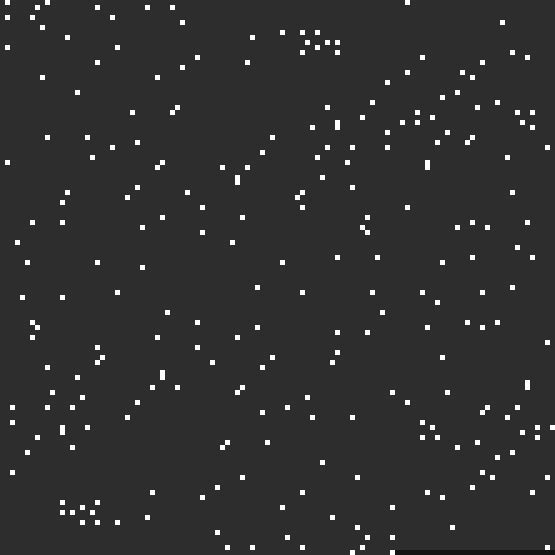
\includegraphics[width=0.7\textwidth]{twiddle_group_in_field.png}
\caption{The 256 \(n\)-th roots of unity modulo the Proth prime \(p = 12289\), the twiddle group of an order-256 transform, lit against the other residues of \(p\). Each point sits at its residue value, placed by an integer row layout with no float, no angle and no geometric circle. The roots are a cyclic group under multiplication, but their residues spread across the field. The group and its order are not visible. A root of half the order, \(\omega^2\) of order 128, generates a proper subgroup and matches the correct root on the identity, the sum, the sum of squares and the sampled group law over the length-\(n\) table; only the order test separates them. Generated by \texttt{proof\_twiddle\_group\_in\_field.py} (PRF-x-014).}
\label{fig:twiddle-group}
\end{figure}

\section{Two silent wrong answers the certificate caught}

The certificate is not hypothetical. Running it caught two failures in this project's own implementation, each of the ordinary shape, neither found by reading the code.

\textbf{A composite modulus, accepted on its shape.} A transform was built on three moduli. The third, \(1610612737\), was accepted because it has the correct Proth shape, \(3 \cdot 2^{29} + 1\), and its generator was raised to \((p-1)/L\) to build a root, with the check beside it confirming only \(\omega^L = 1\), a relation a wrong root also satisfies. No primality certificate was ever produced. The modulus is composite: \(1610612737 = 79 \cdot 20387503\), and Fermat refutes it in one line, \(2^{1610612736} \not\equiv 1 \pmod{1610612737}\), with the witness \(2\). Because the modulus is composite, \(g^{(p-1)/L}\) had no particular order, the twiddles were wrong, and the transform returned numbers of the ordinary shape that were the convolution of nothing. The two correct moduli in the same set returned zero wrong slots out of thirty-two; the composite one returned thirty-two out of thirty-two, and it was noticed only because the three were recombined against each other and disagreed. A shape is not a proof, and a relation the root satisfies is not the order.

\textbf{A width overflow, one level down.} The device transform runs over three moduli, each carrying its Proth witness in the source:

\begin{center}
\begin{tabular}{@{}rlrr@{}}
\toprule
modulus & shape & witness & order \\
\midrule
\(2013265921\) & \(15 \cdot 2^{27} + 1\) & 11 & \(2^{27}\) \\
\(2281701377\) & \(17 \cdot 2^{27} + 1\) & 3 & \(2^{27}\) \\
\(3892314113\) & \(29 \cdot 2^{27} + 1\) & 3 & \(2^{27}\) \\
\bottomrule
\end{tabular}
\end{center}

The first run of that kernel agreed with the host on the first modulus and differed in every slot on the other two. The property separating them is not primality, which all three have. It is that \(2013265921\) is below \(2^{31}\) and the other two are above it. In the butterfly, two residues below a modulus above \(2^{31}\) sum past \(2^{32}\) and wrap, silently, in a type that raises nothing, and the same is true of the borrow in the difference. Only the smallest modulus never reached the boundary. Widened to 64 bits, all three agree with the host at every size tested. This is the same failure as the composite modulus one level down: an unstated assumption about the arithmetic, an output of the ordinary shape, and nothing in it saying otherwise. Both were found by running cases that differ in one property, and the failure named its own cause; neither was found by reading the code.

\section{What it costs, and why the size is ours to choose}

One primality proof is one modular exponentiation. On one desktop, on unbounded integers with nothing vectorized and nothing on the card:

\begin{center}
\begin{tabular}{@{}rrr@{}}
\toprule
bits & decimal digits & one proof \\
\midrule
64 & 19 & \(0.0001\) s \\
128 & 39 & \(0.0001\) s \\
256 & 77 & \(0.0002\) s \\
512 & 154 & \(0.0011\) s \\
1024 & 308 & \(0.0185\) s \\
2048 & 617 & \(0.0419\) s \\
4096 & \(1{,}233\) & \(0.2876\) s \\
\bottomrule
\end{tabular}
\end{center}

A \(1{,}233\) digit number is proved prime in under three tenths of a second, deterministically, with the witness recorded beside it. The cost grows as roughly the square of the bit length, since the exponent has \(N\) bits and each squaring costs the multiply. This is the same theorem the large-prime searches run, where the records are Proth primes of several million digits, and the difference between those runs and this table is only how long one is willing to wait.

The tabled moduli are small because they are sized to a machine word: a lane holds sixty-four bits, a product of two residues has to fit in one, and the modulus therefore stops below \(2^{32}\). That is a property of the lane and not of the mathematics. The arithmetic here is on unbounded integers, the proof runs at any width, and moduli far past anything tabled are produced and proved on demand:

\begin{center}
\begin{tabular}{@{}rlr@{}}
\toprule
modulus & shape & transform length \\
\midrule
\(18446744069414584321\) & \((2^{32}-1) \cdot 2^{32} + 1\) & \(2^{32}\) \\
\(9223372195768565761\) & \(2147483685 \cdot 2^{32} + 1\) & \(2^{32}\) \\
\(39614081257148775820397903873\) & \(140737488355387 \cdot 2^{48} + 1\) & \(2^{48}\) \\
\bottomrule
\end{tabular}
\end{center}

The last admits a transform of length \(281{,}474{,}976{,}710{,}656\). Nobody tables that, because it does not fit in a lane. The floor belongs to the format, and the format is a choice. The certificate is written to run at any width instead of checking a fixed list.

\section{What this refuses}

A modulus outside Proth's range, where \(k\) is not below \(2^n\), since the converse a witness rests on does not hold there. A root whose order falls short of the length asked for, the fiddled twiddle exactly. And any verdict without its certificate: every answer carries the witness establishing it.

\section{Reproduction}

The certificate, both rejections and the half-order floor are reproduced by \texttt{examples/0\_experimental/ntt\_twiddle\_certificate.py} in the public \texttt{anchor\_sift} repository (\texttt{github.com/dstroy0/anchor\_sift}). It re-derives every modulus named here from the factorization of \(p-1\), refuses a composite of Proth shape and a false primitive-root claim by the same checks that pass the real constants, and exhibits a root of half the order passing every \(O(n)\) invariant while the order test alone separates it. It reads no corpus and runs on unbounded Python integers, and every verdict is an exact equality with the witness recorded beside it.

\begin{thebibliography}{9}

\bibitem{proth}
F. Proth.
\emph{Th\'eor\`emes sur les nombres premiers}.
Comptes Rendus de l'Acad\'emie des Sciences, Paris, 87:926, 1878.

\bibitem{ravi}
P. Ravi, B. Yang, S. Bhasin, F. Zhang, A. Chattopadhyay.
\emph{Fiddling the Twiddle Constants: Fault Injection Analysis of the Number Theoretic Transform}.
IACR Transactions on Cryptographic Hardware and Embedded Systems 2023(3); IACR ePrint 2022/824.

\bibitem{kyber}
R. Avanzi, J. Bos, L. Ducas, E. Kiltz, T. Lepoint, V. Lyubashevsky, J. M. Schanck, P. Schwabe, G. Seiler, D. Stehl\'e.
\emph{CRYSTALS-Kyber Algorithm Specifications and Supporting Documentation (version 3.0)}, 2021.

\bibitem{hwang}
V. Hwang, J. Liu, G. Seiler, X. Shi, M.-H. Tsai, B.-Y. Wang, B.-Y. Yang.
\emph{Verified NTT Multiplications for NISTPQC KEM Lattice Finalists: Kyber, SABER, and NTRU}.
IACR Transactions on Cryptographic Hardware and Embedded Systems 2022(4), 718--750.

\bibitem{trieu}
A. Trieu.
\emph{Formally Verified Number-Theoretic Transform}.
IACR Communications in Cryptology 2(4), 2026.

\bibitem{foldntt}
M. Kamba.
\emph{FoldNTT: A Multiplier- and Twiddle-Lean NTT Core with Formally Verified Arithmetic for Proth Primes}.
arXiv:2609.06412, 2026.

\end{thebibliography}

\end{document}
